\documentclass[11pt,a4paper]{article}

\usepackage[utf8]{inputenc}
\usepackage[T1]{fontenc}
\usepackage{amsmath,amssymb,amsthm}
\usepackage{mathtools}
\usepackage{geometry}
\geometry{margin=1in}
\usepackage{tikz}
\usepackage{hyperref}

\newtheorem{theorem}{Theorem}[section]
\newtheorem{definition}[theorem]{Definition}
\newtheorem{example}[theorem]{Example}
\newtheorem{remark}[theorem]{Remark}

\title{From Smooth Manifolds to de Rham Cohomology: An Intuitive Overview}
\author{}
\date{\today}

\begin{document}
    \maketitle

    \begin{abstract}
        Starting with calculus on curved spaces, this talk introduces smooth
        manifolds, differential forms, and de Rham cohomology. We will explore
        how these ideas fit together and how de Rham cohomology connects
        calculus with the topology of a space. The emphasis is on geometric
        intuition and conceptual understanding, with formal definitions kept
        to a minimum. The talk assumes familiarity with multivariable calculus
        and basic linear algebra.
    \end{abstract}

    \section*{Introduction}
    Good afternoon, everyone. My name is Zifan Hua. Today I am going to talk
    about manifolds and de Rham cohomology.

    \section*{Roadmap}
    We will first use small flat maps of Earth to explain how we describe
    individual regions and how overlapping regions fit together. This will
    introduce the idea of manifolds. Then we will describe motion along the
    surface and how a function changes along that motion, leading us to
    tangent and cotangent spaces. Letting these measurements vary smoothly
    across the whole surface leads to differential forms. Finally, we will
    define de Rham cohomology and discuss its significance.

    The aim is to explain the connections and intuition, with the technical
    details intentionally omitted.

    \section{Preliminary Knowledge Expected for the Audience}
    \label{sec:preliminaries}

    Before introducing smooth manifolds, we state the common ground used
    throughout this talk.\footnote{%
        For comprehensive foundational treatments, see
        \cite{lee2013smooth, tu2011introduction}.}

    \begin{enumerate}
        \item \textbf{Euclidean Space $\mathbb{R}^n$}: Euclidean distance,
            open and closed sets.

        \item \textbf{Calculus of Several Variables}:
        \begin{itemize}
            \item Continuity and smoothness ($C^\infty$).
            \item Differentiation: total derivatives, Jacobian matrices,
                and directional derivatives.
            \item Gradient, curl, and divergence.
        \end{itemize}

        \item \textbf{Basic Linear Algebra}.
    \end{enumerate}


    \section{Why Do We Care About Manifolds? A Concrete Example}
    \label{sec:why_manifolds}

    \subsection{A Real-World Motivation: Temperature on Earth}
    \noindent
    \begin{minipage}[c]{0.62\textwidth}
        Consider our planet modeled as a unit 2-sphere in Euclidean 3-space:
        \begin{equation}
            S^2 = \{ x \in \mathbb{R}^3 \mid \|x\| = 1 \}.
        \end{equation}
        Suppose we measure the surface temperature at every point on Earth.
        This defines a continuous (and physically smooth) scalar function:
        \begin{equation}
            f \colon S^2 \to \mathbb{R}.
        \end{equation}
    \end{minipage}\hfill
    \begin{minipage}[c]{0.35\textwidth}
        \centering
        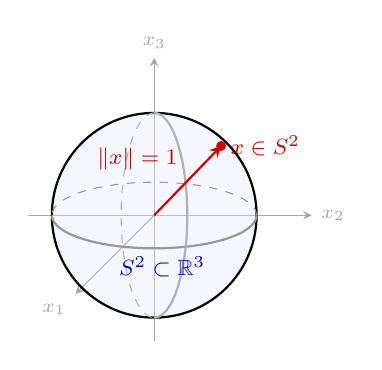
\begin{tikzpicture}[scale=1.0, >=stealth]
  % 3D axes
  \draw[->, gray!70] (-1.6, 0) -- (2.0, 0) node[right, font=\scriptsize] {$x_2$};
  \draw[->, gray!70] (0, -1.6) -- (0, 2.0) node[above, font=\scriptsize] {$x_3$};
  \draw[->, gray!70] (0,0) -- (-1.0, -1.0) node[below left, font=\scriptsize] {$x_1$};
  
  % Sphere
  \draw[thick, fill=blue!10, fill opacity=0.35] (0,0) circle (1.3);
  % Equator
  \draw[dashed, gray!80] (1.3,0) arc (0:180:1.3 and 0.42);
  \draw[thick, gray!80] (-1.3,0) arc (180:360:1.3 and 0.42);
  % Meridian
  \draw[dashed, gray!60] (0,1.3) arc (90:270:0.42 and 1.3);
  \draw[thick, gray!60] (0,1.3) arc (90:-90:0.42 and 1.3);
  
  % Point x on sphere and radius vector
  \draw[->, thick, red!80!black] (0,0) -- (0.85, 0.88) node[midway, above left, font=\footnotesize] {$\|x\|=1$};
  \fill[red!80!black] (0.85, 0.88) circle (1.8pt) node[right, font=\footnotesize] {$x \in S^2$};
  \node[font=\footnotesize, text=blue!80!black] at (0.1, -0.65) {$S^2 \subset \mathbb{R}^3$};
\end{tikzpicture}

    \end{minipage}
    \vspace{0.8em}

    If our goal is purely local, ordinary multivariable calculus from
    Section~\ref{sec:preliminaries} works without issue. However, once we
    study the global behavior of this function across the planet, standard
    calculus in $\mathbb{R}^3$ fails:
    \begin{enumerate}
        \item \textbf{$S^2$ is not an open subset of $\mathbb{R}^3$}:\\
            The standard partial derivative is not defined.
        \item \textbf{Valid directional derivatives must be tangential}:\\
            A legitimate derivative on Earth must measure rates of change
            along directions that are tangent to the surface, rather than
            pointing into the Earth's interior or out into space.
    \end{enumerate}
    That is where manifolds come into place: we need a framework to perform
    calculus directly on curved spaces.

    \subsection{The Intuition: Local Euclidean Approximation}
    The central intuition of a manifold is \textbf{local approximation}. At
    any point $p \in S^2$, a sufficiently small neighborhood $U \subset S^2$
    around $p$ looks like an open region in a flat Euclidean plane
    $\mathbb{R}^2$.

    \begin{figure}[htbp]
        \centering
        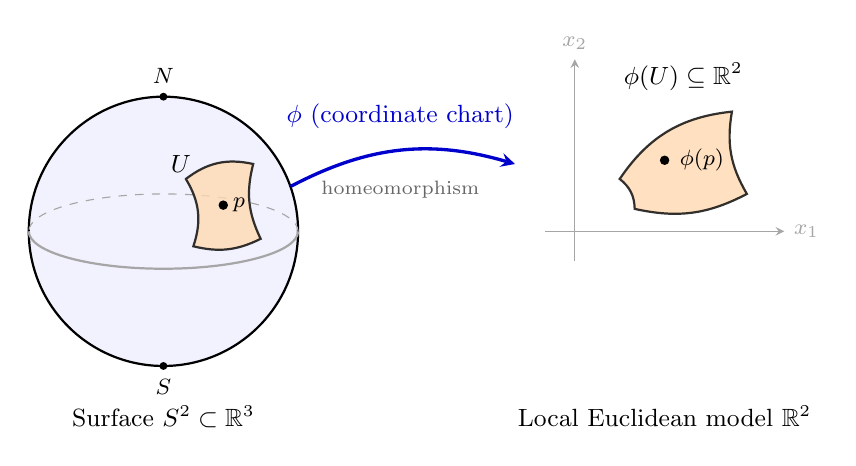
\begin{tikzpicture}[scale=0.95, >=stealth]
  % Left: Sphere S^2
  \begin{scope}[shift={(0,0)}]
    % Sphere outline
    \draw[thick, fill=blue!5] (0,0) circle (1.8);
    % Equator (front solid, back dashed)
    \draw[dashed, gray!70] (1.8,0) arc (0:180:1.8 and 0.5);
    \draw[thick, gray!70] (-1.8,0) arc (180:360:1.8 and 0.5);
    % North and South labels
    \node[above, font=\footnotesize] at (0, 1.85) {$N$};
    \fill (0,1.8) circle (1.5pt);
    \node[below, font=\footnotesize] at (0, -1.85) {$S$};
    \fill (0,-1.8) circle (1.5pt);

    % Local open patch U on sphere
    \draw[thick, fill=orange!30, opacity=0.8] 
      (0.3, 0.7) to[bend left=25] (1.2, 0.9) 
      to[bend right=20] (1.3, -0.1) 
      to[bend left=20] (0.4, -0.2) 
      to[bend right=25] cycle;
    \node[above left, font=\small] at (0.5, 0.65) {$U$};
    \fill (0.8, 0.35) circle (1.8pt) node[right, font=\footnotesize] {$p$};
    \node[below, font=\small] at (0, -2.2) {Surface $S^2 \subset \mathbb{R}^3$};
  \end{scope}

  % Middle: Coordinate chart map phi
  \draw[->, very thick, blue!80!black] (1.7, 0.6) to[bend left=22] 
    node[above=4pt, font=\small] {$\phi$ (coordinate chart)} 
    node[below=7pt, font=\scriptsize, text=gray!80!black] {homeomorphism} (4.7, 0.9);

  % Right: Flat open set in R^2
  \begin{scope}[shift={(5.5,0)}]
    % Axes - crossing at (0,0), clear of the region
    \draw[->, gray!70, thin] (-0.4, 0) -- (2.8, 0) node[right, font=\footnotesize] {$x_1$};
    \draw[->, gray!70, thin] (0, -0.4) -- (0, 2.3) node[above, font=\footnotesize] {$x_2$};
    
    % Flat open region phi(U) placed cleanly in the positive quadrant away from axes
    \draw[thick, fill=orange!30, opacity=0.8] 
      (0.6, 0.7) to[bend left=25] (2.1, 1.6) 
      to[bend right=20] (2.3, 0.5) 
      to[bend left=20] (0.8, 0.3) 
      to[bend right=25] cycle;
      
    % Region label placed comfortably above
    \node[above, font=\small] at (1.45, 1.75) {$\phi(U) \subseteq \mathbb{R}^2$};
    
    % Point phi(p) with label placed centered horizontally inside the orange patch
    \fill (1.2, 0.95) circle (1.8pt) node[right=2pt, font=\footnotesize] {$\phi(p)$};
    
    \node[below, font=\small] at (1.2, -2.2) {Local Euclidean model $\mathbb{R}^2$};
  \end{scope}
\end{tikzpicture}

        \caption{%
            The local coordinate chart: an open neighborhood $U$ on the sphere
            $S^2$ is mapped homeomorphically to an open set $\phi(U) \subseteq
            \mathbb{R}^2$, allowing local calculus on the surface.
        }
        \label{fig:sphere_chart}
    \end{figure}

    \paragraph{Analogy with Algebraic Varieties.}
    An algebraic variety is not globally affine; it is constructed by gluing
    together affine open subsets along regular transition functions.

    \subsection{Constructing \texorpdfstring{$S^2$}{S²} by Gluing Two Disks}
    \label{sec:gluing_s2}

    Here is the picture to keep in mind:
    \begin{enumerate}
        \item Cut one disk from each of two parallel planes.
        \item Bend the disks into two bowls.
        \item Bring the bowls together so they overlap along a narrow strip.
    \end{enumerate}

    \begin{figure}[htbp]
        \centering
        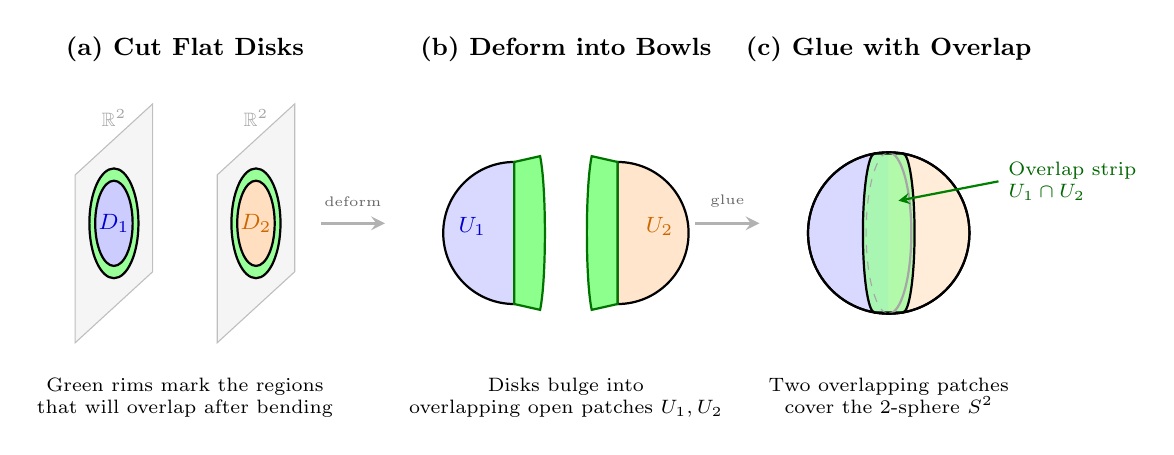
\begin{tikzpicture}[scale=0.82, >=stealth]
  % -------------------------------------------------------------
  % Panel 1: Cut two disks from parallel planes
  % -------------------------------------------------------------
  \begin{scope}[shift={(0,0)}]
    \node[above, font=\bfseries\small] at (1.3, 2.5) {(a) Cut Flat Disks};
    
    % Left plane
    \draw[gray!50, fill=gray!8] (-0.4, -1.7) -- (0.8, -0.6) -- (0.8, 2.0) -- (-0.4, 0.9) -- cycle;
    \node[above, gray!70, font=\scriptsize] at (0.2, 1.5) {$\mathbb{R}^2$};
    % Left disk with a green rim marking the future overlap collar
    \draw[thick, fill=green!40] (0.2, 0.15) ellipse (0.38 and 0.85);
    \draw[thick, fill=blue!20] (0.2, 0.15) ellipse (0.29 and 0.66);
    \node[font=\footnotesize, text=blue!80!black] at (0.2, 0.15) {$D_1$};
    \coordinate (chart-D1) at (0.55,0.15);

    % Right plane
    \draw[gray!50, fill=gray!8] (1.8, -1.7) -- (3.0, -0.6) -- (3.0, 2.0) -- (1.8, 0.9) -- cycle;
    \node[above, gray!70, font=\scriptsize] at (2.4, 1.5) {$\mathbb{R}^2$};
    % Right disk with a matching future overlap collar
    \draw[thick, fill=green!40] (2.4, 0.15) ellipse (0.38 and 0.85);
    \draw[thick, fill=orange!25] (2.4, 0.15) ellipse (0.29 and 0.66);
    \node[font=\footnotesize, text=orange!80!black] at (2.4, 0.15) {$D_2$};
    \coordinate (chart-D2) at (2.75,0.15);

    \node[below, font=\scriptsize, align=center] at (1.3, -2.1) {Green rims mark the regions\\that will overlap after bending};
  \end{scope}

  % Arrow 1 -> 2
  \draw[->, very thick, gray!60] (3.4, 0.15) -- (4.4, 0.15) node[midway, above=2pt, font=\tiny, text=gray!80!black] {deform};

  % -------------------------------------------------------------
  % Panel 2: Deform into overlapping open patches
  % -------------------------------------------------------------
  \begin{scope}[shift={(6.2,0)}]
    \node[above, font=\bfseries\small] at (1.0, 2.5) {(b) Deform into Bowls};

    % Surface strips match the patches in sphere_transition.tex.
    \draw[thick, fill=blue!15]
      (0.2, 1.1) arc (90:270:1.1 and 1.1) -- cycle;
    \path[fill=green!45, draw=green!45!black, thick]
      (0.2,1.1) -- (0.2,-1.1) -- (0.60,-1.19)
      .. controls (0.70,-0.73) and (0.70,0.73) .. (0.60,1.19) -- cycle;
    \node[font=\footnotesize, text=blue!80!black] at (-0.45, 0.1) {$U_1$};
    \coordinate (chart-U1) at (0.0,0.9);
    \coordinate (transition-U1) at (0.5,0.15);

    \draw[thick, fill=orange!20]
      (1.8, 1.1) arc (90:-90:1.1 and 1.1) -- cycle;
    \path[fill=green!45, draw=green!45!black, thick]
      (1.8,1.1) -- (1.8,-1.1) -- (1.40,-1.19)
      .. controls (1.30,-0.73) and (1.30,0.73) .. (1.40,1.19) -- cycle;
    \node[font=\footnotesize, text=orange!80!black] at (2.45, 0.1) {$U_2$};
    \coordinate (chart-U2) at (2.4,0.8);
    \coordinate (transition-U2) at (1.5,0.15);

    \node[below, font=\scriptsize, align=center] at (1.0, -2.1) {Disks bulge into\\overlapping open patches $U_1, U_2$};
  \end{scope}

  % Arrow 2 -> 3
  \draw[->, very thick, gray!60] (9.2, 0.15) -- (10.2, 0.15) node[midway, above=2pt, font=\tiny, text=gray!80!black] {glue};

  % -------------------------------------------------------------
  % Panel 3: Glued together with overlapping strip
  % -------------------------------------------------------------
  \begin{scope}[shift={(12.2,0)}]
    \node[above, font=\bfseries\small] at (0, 2.5) {(c) Glue with Overlap};

    % Left hemisphere (blue)
    \draw[thick, fill=blue!15] (0, 1.25) arc (90:270:1.25);
    
    % Right hemisphere (orange)
    \draw[thick, fill=orange!15] (0, 1.25) arc (90:-90:1.25);

    % Overlapping collar / strip in center (green tint)
    \draw[thick, fill=green!40, fill opacity=0.75] 
      (-0.22, 1.23) arc (90:270:0.18 and 1.23) 
      -- (0.22, -1.23) arc (-90:90:0.18 and 1.23) -- cycle;
      
    % Central boundary curve
    \draw[dashed, gray!70] (0, 1.25) arc (90:270:0.35 and 1.25);
    \draw[thick, gray!70] (0, 1.25) arc (90:-90:0.35 and 1.25);

    % Full sphere circle boundary
    \draw[thick] (0,0) circle (1.25);

    % Callout for overlap placed clearly outside the sphere to the right
    \draw[->, thick, green!50!black] (1.7, 0.8) -- (0.15, 0.5);
    \node[right, font=\scriptsize, align=left, text=green!40!black] at (1.7, 0.8) {Overlap strip\\$U_1 \cap U_2$};

    \node[below, font=\scriptsize, align=center] at (0, -2.1) {Two overlapping patches\\cover the 2-sphere $S^2$};
  \end{scope}

  % The chart-map slide enables these arrows; the original figure omits them.
  \ifdefined\showchartmaps
    \draw[->, very thick, blue!80!black]
      (chart-U1) .. controls +(-0.4,1.8) and +(0.8,2.4) .. (chart-D1)
      node[midway, above=4pt, font=\small] {$\phi_1$};
    \draw[->, very thick, orange!80!black,
        preaction={draw=white,line width=3.5pt}]
      (chart-U2) .. controls +(-1.0,1.9) and +(1.0,2.2) .. (chart-D2)
      node[midway, above=4pt, font=\small] {$\phi_2$};
  \fi

  % A separate variant traces one point through a coordinate transition.
  \ifdefined\showtransitionmaps
    \draw[->, very thick, blue!80!black, shorten <=3pt, shorten >=3pt]
      (chart-D1) .. controls +(0.9,2.2) and +(-0.2,2.2) .. (transition-U1)
      node[midway, above=4pt, font=\small] {$\phi_1^{-1}$};
    \draw[->, very thick, orange!80!black, shorten <=3pt, shorten >=3pt,
        preaction={draw=white,line width=3.5pt}]
      (transition-U2) .. controls +(-0.3,2.0) and +(1.0,2.4) .. (chart-D2)
      node[midway, above=4pt, font=\small] {$\phi_2$};
    \draw[densely dashed, thick, red!80!black, shorten <=4.5pt, shorten >=4.5pt]
      (transition-U1) -- (transition-U2);
    \draw[->, very thick, red!80!black, shorten <=3pt, shorten >=3pt]
      (chart-D1) .. controls +(0.3,-1.65) and +(0.6,-1.65) .. (chart-D2)
      node[midway, below=3pt, font=\small] {$\phi_2\circ\phi_1^{-1}$};
    \foreach \point in {chart-D1,transition-U1,transition-U2,chart-D2}
      \filldraw[fill=red!85!black,draw=white,line width=0.35pt]
        (\point) circle[radius=2.2pt];
    \node[below=10pt,font=\scriptsize,text=red!80!black] at (transition-U1) {$p$};
    \node[below=10pt,font=\scriptsize,text=red!80!black] at (transition-U2) {$p$};
  \fi
\end{tikzpicture}

        \caption{%
            A three-step picture of gluing two disks to form $S^2$. The green
            rims in (a) mark the regions that will overlap after bending.
        }
        \label{fig:sphere_gluing}
    \end{figure}

    \subsection{The Precise Definition of a Smooth Manifold}
    We follow Lee's presentation in Chapter~1, Section ``Smooth Structures,''
    especially pages 11--13 \cite[Chapter~1, ``Smooth Structures,'' pp.~11--
    13]{lee2013smooth}; see also Tu's treatment in Chapter~2
    \cite[Chapter~2]{tu2011introduction}.

    \begin{definition}[Smooth Manifold \cite{lee2013smooth, tu2011introduction}]
        Let $M$ be a Hausdorff, second-countable topological space. These are
        technical assumptions that we will not discuss further; if you are
        unfamiliar with topology, you may think of $M$ as a subspace of some
        $\mathbb{R}^m$.

        A \textbf{coordinate chart} on $M$ is a pair $(U, \phi)$, where $U
        \subseteq M$ is open and $\phi \colon U \to \phi(U) \subseteq
        \mathbb{R}^n$ is a homeomorphism (a continuous bijection with a
        continuous inverse) onto an open subset of $\mathbb{R}^n$.

        Two charts $(U, \phi)$ and $(V, \psi)$ are \textbf{smoothly
        compatible} if either $U \cap V = \emptyset$, or the transition map
        \begin{equation}
            \psi \circ \phi^{-1} \colon \phi(U \cap V) \to \psi(U \cap V)
        \end{equation}
        is a $C^\infty$ diffeomorphism between open subsets of $\mathbb{R}^n$.

        A \textbf{smooth atlas} $\mathcal{A}$ on $M$ is a collection of
        smoothly compatible charts $\{(U_\alpha, \phi_\alpha)\}_{\alpha \in
        I}$ whose domains cover $M$:
        \begin{equation}
            \bigcup_{\alpha \in I} U_\alpha = M.
        \end{equation}
        A \textbf{smooth $n$-manifold} is a Hausdorff, second-countable
        topological space $M$ together with a smooth atlas of dimension $n$.
    \end{definition}

    \subsection{Checking the Gluing Example Against the Definition}

    Return to Figure~\ref{fig:sphere_gluing}. It shows the two bowl-shaped
    patches and the band where they overlap. In
    Figure~\ref{fig:sphere_transition}, the same overlap is drawn on both
    patches: the green strip on the left patch corresponds to the green strip
    on the right. The arrows show points in one strip mapping to corresponding
    points in the other. This is the transition function, and it describes how
    we glue the two patches together.

    The condition in the definition is that this transition be smooth.

    \begin{figure}[htbp]
        \centering
        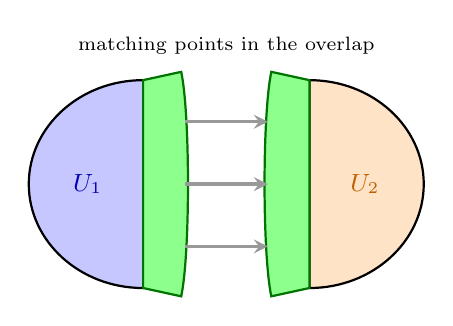
\begin{tikzpicture}[>=stealth, scale=0.88]
  % Two overlapping open patches, each with a collar along its full flat edge
  \draw[thick, fill=blue!22] (-1.2,1.5) arc (90:270:1.65 and 1.5) -- cycle;
  \path[fill=green!45, draw=green!45!black, thick]
    (-1.2,1.5) -- (-1.2,-1.5) -- (-0.65,-1.62)
    .. controls (-0.52,-1.0) and (-0.52,1.0) .. (-0.65,1.62) -- cycle;

  \draw[thick, fill=orange!22] (1.2,1.5) arc (90:-90:1.65 and 1.5) -- cycle;
  \path[fill=green!45, draw=green!45!black, thick]
    (1.2,1.5) -- (1.2,-1.5) -- (0.65,-1.62)
    .. controls (0.52,-1.0) and (0.52,1.0) .. (0.65,1.62) -- cycle;

  \node[font=\small, text=blue!70!black] at (-2.0,0) {$U_1$};
  \node[font=\small, text=orange!75!black] at (2.0,0) {$U_2$};
  \node[font=\scriptsize] at (0,2.0) {matching points in the overlap};

  % Arrows pair points all along the two full-edge overlap collars
  \draw[->, very thick, gray!80] (-0.6,0.9) -- (0.6,0.9);
  \draw[->, very thick, gray!80] (-0.6,0) -- (0.6,0);
  \draw[->, very thick, gray!80] (-0.6,-0.9) -- (0.6,-0.9);
\end{tikzpicture}

        \caption{%
            Two hemispherical patches, with matching green overlap strips.
            Arrows show corresponding points being mapped from the left strip
            to the right.
        }
        \label{fig:sphere_transition}
    \end{figure}

    \subsection{The Benefit: Uniting Local Calculus with Global Coherence}
    Why is this definition so effective?
    \begin{itemize}
        \item \textbf{Locally}:\\
            We can calculate using standard multivariable calculus from
            Section~\ref{sec:preliminaries} by pulling functions and vectors
            back to open subsets of $\mathbb{R}^n$ via charts. No new
            computational mechanics are needed.
        \item \textbf{Globally}:\\
            Because the transition maps $\psi \circ \phi^{-1}$ are smooth
            diffeomorphisms, the multivariate chain rule guarantees that all
            calculus operations (smoothness of functions, directional
            derivatives, vector fields, and differential forms) are
            coordinate-independent.
    \end{itemize}
    This allows us to study global derivatives, PDEs on curved geometries,
    optimization on manifolds, and global topological invariants (such as de
    Rham cohomology) rigorously.


    \section{Tangent and Cotangent Spaces}
    \label{sec:tangent-cotangent}

    We now want to differentiate functions on a manifold. For temperature on
    Earth, this means choosing a direction of motion and measuring the rate
    of temperature change along it. Tangent spaces describe the possible
    directions, while cotangent spaces describe linear measurements of them.

    \subsection{Tangent Vectors as Velocities of Curves}
    Directional derivatives begin with a direction at a point. Let $p$ be a
    point on the sphere $S^2\subset\mathbb{R}^3$, and let $v\in\mathbb{R}^3$
    be a nonzero vector based at $p$ and lying in its geometric tangent plane.
    In ordinary multivariable calculus, we measure how a function changes
    along the straight line $p+tv$. But this line leaves the sphere as soon
    as $t\ne0$, so a function defined only on the sphere has no values there
    (Figure~\ref{fig:sphere_direction}).

    \begin{figure}[!ht]
        \centering
        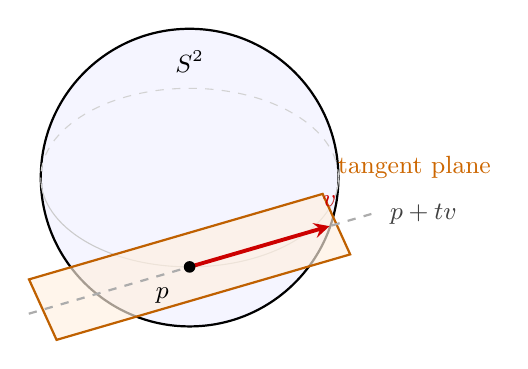
\begin{tikzpicture}[>=stealth, scale=1.05,
    x={(1.8cm,0cm)}, y={(0cm,1.44cm)}, z={(0cm,-1.08cm)}]
  % Use the same sphere projection as the curve-velocity figure.
  \draw[thick, fill=blue!4] (0,0) circle[radius=1.8cm];
  \draw[gray!35, dashed] (1.8cm,0cm) arc (0:180:1.8cm and 1.08cm);
  \draw[gray!40] (-1.8cm,0cm) arc (180:360:1.8cm and 1.08cm);
  \node[font=\small] at (0cm,1.4cm) {$S^2$};

  % The affine plane z=1 is tangent at p=(0,0,1).
  \filldraw[fill=orange!12, fill opacity=0.65,
      draw=orange!75!black, thick]
    (-0.894,-0.613,1) -- (1.079,0.105,1) --
    (0.894,0.613,1) -- (-1.079,-0.105,1) -- cycle;
  \node[font=\small, text=orange!80!black, above right=2pt]
    at (0.894,0.613,1) {tangent plane};

  % The tangent line lies in the plane and leaves the sphere away from p.
  \draw[gray!65, dashed, thick]
    ({-1.15*cos(20)},{-1.15*sin(20)},1) --
    ({1.30*cos(20)},{1.30*sin(20)},1)
    node[right=3pt, font=\small, text=black!75] {$p+tv$};
  \draw[->, red!80!black, line width=1.4pt]
    (0,0,1) -- ({cos(20)},{sin(20)},1)
    node[above=3pt, font=\small] {$v$};
  \fill (0,0,1) circle[radius=2pt];
  \node[font=\small, below left=4pt] at (0,0,1) {$p$};
\end{tikzpicture}

        \caption{%
            The vector $v$ lies in the tangent plane at $p$, but the straight
            line $p+tv$ leaves the sphere. To describe motion on the sphere,
            we use a curve on its surface.
        }
        \label{fig:sphere_direction}
    \end{figure}

    The idea is to replace the straight line $p+tv$ with a curve that stays
    on the manifold. On a smooth manifold $M$, consider a smooth curve
    \begin{equation}
        \gamma\colon(-\epsilon,\epsilon)\to M,\qquad\gamma(0)=p.
    \end{equation}
    Given a smooth function $f\colon M\to\mathbb{R}$, the composition is an
    ordinary function of one variable:
    \[
        f\circ\gamma\colon(-\epsilon,\epsilon)\to\mathbb{R},
        \qquad t\mapsto f(\gamma(t)).
    \]
    We can therefore measure how $f$ changes along the curve by taking
    \begin{equation}
        \left.\frac{d}{dt}\right|_{t=0}f(\gamma(t)).
    \end{equation}
    In the Euclidean case $M=\mathbb{R}^n$, choosing the straight-line curve
    $\gamma(t)=p+tv$ gives the familiar directional derivative:
    \begin{equation}
        \left.\frac{d}{dt}\right|_{t=0}f(\gamma(t))
        =\left.\frac{d}{dt}\right|_{t=0}f(p+tv)=D_vf(p).
    \end{equation}

    But there are many different smooth curves through $p$. An entire curve
    carries more
    information than we need: different paths can have the same initial
    direction and speed. We therefore group such curves together.
    Following Lee \cite[p.~72]{lee2013smooth}, we say two curves $\gamma_1$ and
    $\gamma_2$ are equivalent ($\gamma_1\sim\gamma_2$) if they produce the same
    rate of change for every smooth test function
    $f\colon M\to\mathbb{R}$:\footnote{%
        Lee discusses curve classes as an alternative to his definition using
        derivations, and uses smooth test functions defined near $p$.
        Multiplying such a function by a smooth bump function equal to $1$
        near $p$ and supported in its domain, then extending by zero, gives a
        global smooth function that agrees with it near $p$ and has the same
        derivatives along curves through $p$; see
        \cite[Proposition~2.25]{lee2013smooth}. Thus, the local and global
        test-function formulations are equivalent.}
    \begin{equation}
        \left.\frac{d}{dt}\right|_{t=0}f(\gamma_1(t))
        =\left.\frac{d}{dt}\right|_{t=0}f(\gamma_2(t)).
    \end{equation}
    Geometrically, the curves have the same initial velocity at $p$
    (Figure~\ref{fig:sphere_tangent}).

    \begin{figure}[!ht]
        \centering
        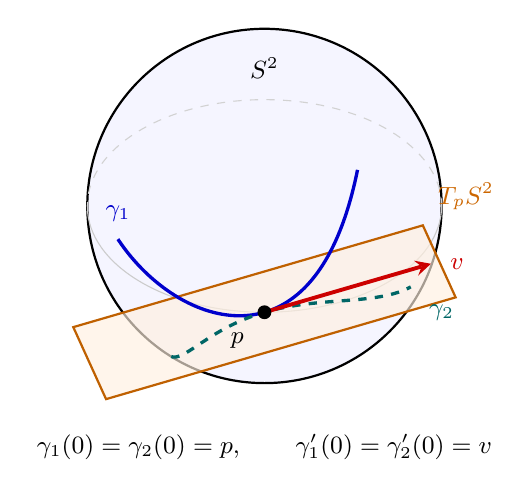
\begin{tikzpicture}[>=stealth, scale=1.25,
    x={(1.8cm,0cm)}, y={(0cm,1.44cm)}, z={(0cm,-1.08cm)}]
  % Orthographic projection of the unit sphere: (x,y,z) -> (1.8x,1.44y-1.08z).
  \draw[thick, fill=blue!4] (0,0) circle[radius=1.8cm];
  \draw[gray!35, dashed] (1.8cm,0cm) arc (0:180:1.8cm and 1.08cm);
  \draw[gray!40] (-1.8cm,0cm) arc (180:360:1.8cm and 1.08cm);
  \node[font=\small] at (0cm,1.4cm) {$S^2$};

  % A patch of the actual tangent plane z=1 at p=(0,0,1).
  \filldraw[fill=orange!12, fill opacity=0.65,
      draw=orange!75!black, thick]
    (-0.894,-0.613,1) -- (1.079,0.105,1) --
    (0.894,0.613,1) -- (-1.079,-0.105,1) -- cycle;
  \node[font=\small, text=orange!80!black, above right=2pt]
    at (0.894,0.613,1) {$T_pS^2$};

  % In a rotated tangent basis e1,e2, use
  % gamma_i(t)=t e1 +/- 0.85 t^2 e2 + sqrt(1-t^2-0.85^2 t^4) p.
  % Both lie on S^2, pass through p, and have derivative e1 at t=0.
  \draw[blue!80!black, very thick]
    plot[domain=-0.72:0.72, samples=101, variable=\t]
    ({cos(20)*\t-sin(20)*0.85*\t*\t},
     {sin(20)*\t+cos(20)*0.85*\t*\t},
     {sqrt(1-\t*\t-0.85*0.85*\t*\t*\t*\t)});
  \draw[teal!80!black, very thick, dashed]
    plot[domain=-0.72:0.72, samples=101, variable=\t]
    ({cos(20)*\t+sin(20)*0.85*\t*\t},
     {sin(20)*\t-cos(20)*0.85*\t*\t},
     {sqrt(1-\t*\t-0.85*0.85*\t*\t*\t*\t)});

  % Labels sit beside separated portions of the curves.
  \node[font=\small, text=blue!80!black, above=3pt]
    at (-0.827,0.168,0.537) {$\gamma_1$};
  \node[font=\small, text=teal!80!black, below right=3pt]
    at (0.827,-0.168,0.537) {$\gamma_2$};

  \draw[->, red!80!black, line width=1.4pt]
    (0,0,1) -- ({cos(20)},{sin(20)},1)
    node[right=3pt, font=\small] {$v$};
  \fill (0,0,1) circle[radius=2pt];
  \node[font=\small, below left=4pt] at (0,0,1) {$p$};
  \node[font=\small, align=center] at (0cm,-2.45cm)
    {$\gamma_1(0)=\gamma_2(0)=p,\qquad
       \gamma_1'(0)=\gamma_2'(0)=v$};
\end{tikzpicture}

        \caption{%
            Two distinct curves $\gamma_1$ and $\gamma_2$ pass through $p$
            with the same velocity vector, defining the same tangent vector
            $v=[\gamma_1]=[\gamma_2]\in T_pS^2$. The blue solid curve and
            green dashed curve take different paths but share the red
            velocity arrow at $p$.
        }
        \label{fig:sphere_tangent}
    \end{figure}

    \begin{definition}[Tangent Vector and Tangent Space \cite{lee2013smooth}]
        A \textbf{tangent vector} at $p\in M$ is an equivalence class of smooth
        curves through $p$, denoted $v=[\gamma]$. The \textbf{tangent space}
        $T_pM$ is the set of all such tangent vectors at $p$.
    \end{definition}

    Although adding curves directly on a curved manifold is not defined,
    $T_pM$ has the structure of an $n$-dimensional real vector space
    \cite[Problem~3-8, p.~76; Proposition~3.10, p.~57]{lee2013smooth}.
    When $M$ is a surface in $\mathbb{R}^3$, it is the familiar tangent plane
    drawn at $p$.

    For Euclidean space viewed as a manifold, we naturally identify
    \[
        T_p\mathbb{R}^n\cong\mathbb{R}^n.
    \]
    A vector $v\in\mathbb{R}^n$ is represented by the straight-line curve
    $\gamma(t)=p+tv$. This explains why an ordinary vector can serve as the
    direction of a directional derivative.

    \subsection{Cotangent Spaces}
    We have described directions of motion. Now we want to measure how a
    function changes in each direction. A rule that assigns a number to each
    tangent vector, linearly in that vector, is a \textbf{cotangent vector};
    that is, a linear map $T_pM\to\mathbb{R}$.
    The \textbf{cotangent space} $T_p^*M$ is the linear dual of the tangent
    space:\footnote{%
        Here, $\operatorname{Hom}_{\mathbb{R}}(T_pM,\mathbb{R})$ denotes the
        vector space of all linear maps from $T_pM$ to $\mathbb{R}$, the dual
        space recalled in Section~\ref{sec:preliminaries}.}
    \begin{equation}
        T_p^*M=\operatorname{Hom}_{\mathbb{R}}(T_pM,\mathbb{R}).
    \end{equation}
    A natural example is the \textbf{differential} of a smooth function
    $f\colon M\to\mathbb{R}$ at $p$. It measures the rate of change along a
    curve representing the tangent vector:
    \begin{equation}
        df_p([\gamma])=\left.\frac{d}{dt}\right|_{t=0}f(\gamma(t)).
    \end{equation}

    \paragraph{Intuition: $df_p$ Corresponds to the Gradient $\nabla f(p)$.}
    In multivariable calculus, the directional derivative can be calculated
    by taking the dot product of the gradient with a direction $v$. The vector
    $\nabla f(p)$ therefore determines a linear functional:
    \[
        \nabla f(p)\cdot(-)\colon\mathbb{R}^n\to\mathbb{R},
        \qquad v\mapsto\nabla f(p)\cdot v.
    \]
    Since $T_p\mathbb{R}^n$ is identified with $\mathbb{R}^n$, this functional
    is a cotangent vector. Choosing $\gamma(t)=p+tv$ in the manifold definition
    gives the same calculation:
    \begin{equation}
        df_p([\gamma])
        =\left.\frac{d}{dt}\right|_{t=0}f(p+tv)
        =\nabla f(p)\cdot v.
    \end{equation}
    Thus, $df_p$ is exactly the linear functional represented by the Euclidean
    gradient:
    \[
        df_p=\nabla f(p)\cdot(-).
    \]


    \section{Differential Forms and the Exterior Derivative}
    \label{sec:forms-derivative}

    \subsection{Differential 1-Forms}
    In the previous section, we introduced the cotangent space $T_p^*M$ at a
    point $p$. Each element of this space is a linear map that takes a tangent
    velocity at $p$ and returns a real number.\footnote{%
        For an alternative, informal introduction to differential forms from
        the viewpoint of integration, see Tao \cite{tao2007differential}.
        The PDF link is included in the bibliography.}

    A \textbf{differential $1$-form} $\omega$ on $M$ assigns a cotangent
    vector $\omega_p \in T_p^*M$ to every point $p$, with this assignment
    varying smoothly from point to point.\footnote{%
        We leave the precise meaning of ``varying smoothly'' as a technical
        detail.} Thus, at each point, we have a
    linear measurement
    \begin{equation}
        \omega_p \colon T_pM \to \mathbb{R}.
    \end{equation}

    We already have an example: the differential $df_p$ at each point.
    Assigning these differentials across the manifold gives the $1$-form $df$.
    \textbf{Thus, $df_p$ is a measurement at one point, while $df$ provides
    these measurements throughout the manifold.}

    Returning to temperature on the sphere, $df_p([\gamma])$ tells us how
    quickly the temperature changes as a particle passes through $p$ along
    $\gamma$. The $1$-form $df$ provides this temperature-change measurement
    everywhere on the sphere.

    \paragraph{Vector Fields and $1$-Forms in Euclidean Space.}
    Recall that at each $p \in \mathbb{R}^n$, the cotangent vector $df_p$ corresponds
    to the vector $\nabla f(p)$ under the Euclidean dot-product identification:
    $df_p(v) = \nabla f(p) \cdot v$. Applying this at every point, the
    $1$-form $df$ corresponds to the gradient vector field $\nabla f$.
    More generally, any smooth vector field $F$ on $\mathbb{R}^n$ defines an
    associated $1$-form $\omega_F$ by
    \begin{equation}
        (\omega_F)_p(v) = F(p) \cdot v, \qquad v \in T_p\mathbb{R}^n = \mathbb{R}^n.
    \end{equation}
    Thus $df = \omega_{\nabla f}$. If $F$ is a force field and $v$ is a unit
    direction, $(\omega_F)_p(v)$ is the force component in that direction.

    \subsection{Geometric Motivation for Higher Forms}
    A $1$-form can measure change along a single tangent direction, as $df$
    does. To measure quantities associated with an area, as in the study of
    curl, we use higher forms. A $2$-form takes two tangent vectors
    $v,w \in T_pM$ and gives a signed measurement of the parallelogram they span. Swapping the vectors changes the sign of this measurement,
    just as swapping the vectors in a cross product in $\mathbb{R}^3$
    changes its sign:
    \[
        \omega_p(v,w) = -\omega_p(w,v).
    \]

    \subsection{Multilinear and Alternating Maps}
    To describe these measurements, we use multilinear and alternating maps
    on a vector space $V$, following Munkres \cite[\S26, p.~220;
    \S27, pp.~229--230]{munkres1991analysis}.

    \begin{definition}[Multilinear and Alternating Maps %
        \cite{munkres1991analysis}]
        Let $V$ be a real vector space. A map
        \[
            T \colon \underbrace{V \times \dots \times V}_{k \text{ copies}}
            \to \mathbb{R}
        \]
        is \textbf{multilinear of degree $k$} (or a \textbf{$k$-linear map}) if
        it is linear in each argument when all other $k-1$ arguments are held
        fixed.

        A multilinear map $T$ of degree $k$ is \textbf{alternating} if swapping
        any two distinct arguments reverses its sign: for any $1 \le i < j \le
        k$,
        \begin{equation}
            T(v_1, \dots, v_i, \dots, v_j, \dots, v_k)
            = -T(v_1, \dots, v_j, \dots, v_i, \dots, v_k).
        \end{equation}
        Consequently, if any two input vectors are identical ($v_i = v_j$ for
        $i \neq j$), an alternating map necessarily evaluates to zero:
        $T(\dots, v, \dots, v, \dots) = 0$.
    \end{definition}

    \subsection{Higher Differential Forms: At a Point and Globally}
    We can now define differential forms of arbitrary degree $k$ on a
    manifold, following Lee \cite[``Differential Forms on Manifolds,''
    pp.~359--360]{lee2013smooth}:
    \begin{enumerate}
        \item \textbf{At a single point $p \in M$}:\\
            A \textbf{$k$-form at $p$} is an alternating multilinear map on
            the tangent space $T_pM$:
            \[
                \omega_p \colon
                \underbrace{T_pM \times \dots \times T_pM}_{k \text{ copies}}
                \to \mathbb{R}.
            \]
        \item \textbf{On the manifold $M$ as a whole}:\\
            A \textbf{differential $k$-form} $\omega$ on $M$ is a smooth
            choice of an alternating multilinear map at each point
            \cite[p.~360]{lee2013smooth}.\footnote{%
                As with $1$-forms, ``smooth choice'' is an informal
                description; we do not formalize this notion in the talk.}
    \end{enumerate}

    We denote the space of smooth $k$-forms on $M$ by $\Omega^k(M)$, with
    $\Omega^0(M) = C^\infty(M)$ (smooth scalar functions).
    This is a real vector space: we add forms and multiply them by real
    scalars point by point. For $\omega,\omega' \in \Omega^k(M)$,
    $a \in \mathbb{R}$, and $v_1,\dots,v_k \in T_pM$,
    \[
        \begin{aligned}
            (\omega_p+\omega'_p)(v_1,\dots,v_k)
                &= \omega_p(v_1,\dots,v_k)+\omega'_p(v_1,\dots,v_k), \\
            (\omega+\omega')_p &= \omega_p+\omega'_p, \\
            (a\omega)_p &= a\omega_p.
        \end{aligned}
    \]
    Sums and scalar multiples remain smooth and alternating.

    \subsection{The Exterior Derivative}
    The differential of a smooth function turns a $0$-form into a $1$-form.
    This operation extends to differential forms of every degree through an
    operator called the \textbf{exterior derivative}:
    \begin{equation}
        d \colon \Omega^k(M) \to \Omega^{k+1}(M).
    \end{equation}
    We omit its construction (see \cite[Theorem~14.24, pp.~365--366]{lee2013smooth})
    and retain three properties needed for this talk:
    \begin{enumerate}
        \item \textbf{Linearity}:\\
            For $a,b \in \mathbb{R}$ and $\alpha,\beta \in \Omega^k(M)$,
            \[
                d(a\alpha + b\beta) = a\,d\alpha + b\,d\beta.
            \]
        \item \textbf{On functions}:\\
            For a smooth function $f$, $df$ is the differential introduced in
            Section~\ref{sec:tangent-cotangent}.
        \item \textbf{Differentiating twice gives zero}:\\
            For every differential form $\omega$,
            \[
                d(d\omega) = 0, \qquad \text{that is, } d^2 = 0.
            \]
    \end{enumerate}

    In $\mathbb{R}^3$, the successive exterior derivatives correspond to the
    familiar vector-calculus operators:
    \[
        \begin{aligned}
            d &\colon C^\infty(\mathbb{R}^3) \to \Omega^1(\mathbb{R}^3)
                &&\text{gradient}, \\
            d &\colon \Omega^1(\mathbb{R}^3) \to \Omega^2(\mathbb{R}^3)
                &&\text{curl}, \\
            d &\colon \Omega^2(\mathbb{R}^3) \to \Omega^3(\mathbb{R}^3)
                &&\text{divergence}.
        \end{aligned}
    \]
    The first map sends $f$ to $df$, which we already identified with the
    gradient in Section~\ref{sec:tangent-cotangent}. These are the familiar
    vector-calculus operators expressed in the language of differential forms
    on the manifold $\mathbb{R}^3$.\footnote{%
        For the precise identifications, see Lee
        \cite[Equation~(14.27), p.~368; Exercise~14.28]{lee2013smooth}.
        For explicit formulas, see also Bouchard
        \cite[\S4.4.1, Definitions~4.4.1--4.4.3 and
        Table~4.4.8]{bouchard_exterior_vector}.}

    There are no nonzero forms of degree greater than $3$ on $\mathbb{R}^3$;
    in particular, $\Omega^4(\mathbb{R}^3)=\{0\}$.\footnote{%
        Any four vectors in a three-dimensional tangent space are linearly
        dependent, so every alternating $4$-linear form vanishes. The same
        argument applies to all higher degrees.}
    Thus, the next map $d\colon\Omega^3(\mathbb{R}^3)\to\Omega^4(\mathbb{R}^3)$
    is zero.

    The familiar identities
    \[
        \operatorname{curl}(\nabla f) = 0,
        \qquad
        \operatorname{div}(\operatorname{curl} F) = 0
    \]
    are instances of $d^2 = 0$. This identity is the starting point for de Rham
    cohomology.


    \section{de Rham Cohomology: Bridging Geometry, Topology, and Physics}
\label{sec:de_rham}

We now return to the reverse question. In ordinary vector calculus, every
gradient field is curl-free. Does every curl-free field come from a globally
defined scalar potential?

Differential forms let us ask the same question on a manifold. Given a
differential $1$-form $\omega$, can we find a smooth function $f$, defined on
the whole manifold, such that
\begin{equation}
    \omega = df?
\end{equation}
Since $d^2 = 0$, such a form must satisfy $d\omega = 0$. We call forms
satisfying this condition \textbf{closed}, and forms that can be written as
$df$ \textbf{exact}. Every exact form is closed, but the converse can fail.

The first \textbf{de Rham cohomology} space records this failure. More
generally, de Rham cohomology asks, at each degree, which closed forms can be
obtained by differentiating a form of one lower degree.

\subsection{Cohomology Groups}
\begin{definition}[de Rham Cohomology Groups]
    For each $k \ge 0$, the \textbf{$k$-th de Rham cohomology group} of $M$ is
    the quotient vector space \cite[p.~441]{lee2013smooth}\footnote{%
        We take $\Omega^{-1}(M)=\{0\}$, so the denominator in degree zero
        is $\{0\}$.}
    \begin{equation}
        H^k_{\mathrm{dR}}(M)
        = \frac{\{\text{closed }k\text{-forms on }M\}}
               {\{\text{exact }k\text{-forms on }M\}}
        = \frac{\ker\!\left(d\colon\Omega^k(M)\to\Omega^{k+1}(M)\right)}
               {\operatorname{im}\!\left(d\colon\Omega^{k-1}(M)\to\Omega^k(M)\right)}.
    \end{equation}
\end{definition}

Since $d$ is linear and $d^2=0$, exact $k$-forms form a linear subspace of
closed $k$-forms. We can therefore define their quotient.

% OPTIONAL BEGIN: Cohomology of Spheres
%\subsection{Cohomology of Spheres}
%While we do not have time in this talk to perform the full calculation, the de
%Rham cohomology groups of the $n$-dimensional sphere $S^n$, for $n \ge 1$,
%are known \cite[Theorem~17.21, p.~450]{lee2013smooth} and illustrate the
%topological meaning of the invariants:
%\begin{equation}
%    H^k_{\mathrm{dR}}(S^n) =
%    \begin{cases}
%        \mathbb{R}, & k = 0 \text{ or } k = n, \\[4pt]
%        0, & 0 < k < n.
%    \end{cases}
%\end{equation}
%These results illustrate how cohomology records different information at
%different degrees. More generally, if two smooth manifolds have different de
%Rham cohomology spaces in some degree, they cannot be diffeomorphic
%\cite[Corollary~17.4, p.~442]{lee2013smooth}.
% OPTIONAL END: Cohomology of Spheres

\subsection{The de Rham Theorem: A Bridge Between Geometry and Topology}
The significance of de Rham cohomology is crystallized by a landmark result in
differential topology (see \cite[Proposition~18.13, pp.~482--483;
Theorem~18.14, p.~484]{lee2013smooth}):

\begin{theorem}[de Rham]
    \label{thm:de_rham}
    For every smooth manifold $M$ and nonnegative integer $k$, there is a
    natural isomorphism of real vector spaces:
    \begin{equation}
        H^k_{\mathrm{dR}}(M) \cong H^k(M; \mathbb{R}),
    \end{equation}
    where $H^k(M; \mathbb{R})$ denotes singular cohomology with real
    coefficients, defined from the topology of $M$ alone.
\end{theorem}

Intuitively, topologists study holes using geometric loops and membranes,
and analogous objects in higher dimensions. Differential forms give us
another way to study them.

The de Rham theorem says that de Rham cohomology recovers exactly the same
information about holes as topological cohomology with real coefficients.
Thus, we can study this topological information through smooth differential
forms and the exterior derivative. The result depends on the topology of the
manifold, even though its definition uses calculus.

\subsection{Physical Significance: Conservative Vector Fields and Topology}
Beyond pure topology, de Rham cohomology plays a decisive role in physics,
explaining theorems that frequently appear mysterious in standard
multivariable calculus courses.

Recall the classical conservative vector field theorem: \emph{on a simply
connected domain $X \subseteq \mathbb{R}^3$, a smooth vector field $F$
satisfies $\operatorname{curl} F = 0$ if and only if $F = \nabla f$ for some
scalar potential $f \colon X \to \mathbb{R}$}
\cite[Corollary~16.27, p.~421]{lee2013smooth}.

\begin{remark}
    If you are unfamiliar with the formal topological definition of ``simply
    connected'', you may simply think of a general well-behaved region in
    $\mathbb{R}^3$ without holes or missing axes (for example, all of
    $\mathbb{R}^3$ or a solid ball).
\end{remark}

Under the dictionary between vector calculus and differential forms:
\begin{enumerate}
    \item $\operatorname{curl} F = 0$ translates to $d\omega_F = 0$, meaning
        that the associated $1$-form $\omega_F$ is \textbf{closed}.
    \item $F = \nabla f$ translates to $\omega_F = df$, meaning that the
        $1$-form is \textbf{exact}.
\end{enumerate}

Thus, the physics theorem that every curl-free field is conservative on $X$ is
precisely the mathematical statement that every closed $1$-form is exact,
which means that the first de Rham cohomology group vanishes:
\begin{equation}
    H^1_{\mathrm{dR}}(X) = 0.
\end{equation}
For a simply connected domain $X$, topology gives $H^1(X; \mathbb{R}) = 0$
\cite[p.~472; Problem~18-2, p.~487]{lee2013smooth}.
The de Rham theorem (Theorem~\ref{thm:de_rham}) then gives
$H^1_{\mathrm{dR}}(X) = 0$, so every closed $1$-form is exact. In
vector-calculus terms, every curl-free field on $X$ has a globally defined
scalar potential. Thus, the question we began with---whether given rates of
change come from one global function---can be answered through topology.


    \section*{Acknowledgments}
    AI was used in typesetting and structuring this manuscript and the
    accompanying presentation slides. Every part of the mathematics is written
    by hand.

    \bibliographystyle{alpha}
    \bibliography{../references}

\end{document}
